% !TEX TS-program = pdflatex
% !TEX encoding = UTF-8 Unicode

% This is a simple template for a LaTeX document using the "article" class.
% See "book", "report", "letter" for other types of document.

\documentclass[16pt]{article} % use larger type; default would be 10pt

\usepackage[utf8]{inputenc} % set input encoding (not needed with XeLaTeX)
\usepackage[T1]{fontenc}
\usepackage{graphicx}
%%% Examples of Article customizations
% These packages are optional, depending whether you want the features they provide.
% See the LaTeX Companion or other references for full information.

%%% PAGE DIMENSIONS
\usepackage{geometry} % to change the page dimensions
\geometry{a4paper} % or letterpaper (US) or a5paper or....
% \geometry{margin=2in} % for example, change the margins to 2 inches all round
% \geometry{landscape} % set up the page for landscape
%   read geometry.pdf for detailed page layout information

\usepackage{graphicx} % support the \includegraphics command and options
\usepackage{listings}
% \usepackage[parfill]{parskip} % Activate to begin paragraphs with an empty line rather than an indent

%%% PACKAGES
\usepackage{booktabs} % for much better looking tables
\usepackage{array} % for better arrays (eg matrices) in maths
\usepackage{paralist} % very flexible & customisable lists (eg. enumerate/itemize, etc.)
\usepackage{verbatim} % adds environment for commenting out blocks of text & for better verbatim
\usepackage{subfig} % make it possible to include more than one captioned figure/table in a single float
% These packages are all incorporated in the memoir class to one degree or another...

%%% HEADERS & FOOTERS
\usepackage{fancyhdr} % This should be set AFTER setting up the page geometry
\pagestyle{fancy} % options: empty , plain , fancy
\renewcommand{\headrulewidth}{0pt} % customise the layout...
\lhead{}\chead{}\rhead{}
\lfoot{}\cfoot{\thepage}\rfoot{}

%%% SECTION TITLE APPEARANCE
\usepackage{sectsty}
\allsectionsfont{\sffamily\mdseries\upshape} % (See the fntguide.pdf for font help)
% (This matches ConTeXt defaults)

%%% ToC (table of contents) APPEARANCE
\usepackage[nottoc,notlof,notlot]{tocbibind} % Put the bibliography in the ToC
\usepackage[titles,subfigure]{tocloft} % Alter the style of the Table of Contents
\renewcommand{\cftsecfont}{\rmfamily\mdseries\upshape}
\renewcommand{\cftsecpagefont}{\rmfamily\mdseries\upshape} % No bold!

%%% END Article customizations

%%% The "real" document content comes below...

\title{Metody Obliczeniowe}
\author{Mateusz Miotk\\ Michał Kulesz\\ Sylwia Kaczmarczyk}
\date{} % Activate to display a given date or no date (if empty),
         % otherwise the current date is printed 

\begin{document}
\maketitle

\section{Treść zadania}

\textbf {Zadanie 1.14}: Ustalić naturalną $n_{max}$. Wczytać $ n \in \lbrace1,2,...,n_{max}\rbrace$, różne węzły $x_1.x_2,...,x_n $ oraz 
dowolne wartości $A_1,A_2,...,A_n$ i $B_1,B_2,...,B_n $. Wyznaczyć w postaci Newtona wielomian interpolacyjny Hermite'a $W = W(x)$ stopnia co najwyżej
$(2n-1)$ spełniający warunki: $W(x_i) = A_i$ oraz $W'(x_i) = B_i$ dla $i = 1,2,...,n$. Wynik przedstawić również w postaci ogólnej.

%\subsection{A subsection}
\section{Podstawa teoretyczna}
\subsection {Wielomian w postaci Newtona:}
Wielomian $p_k(x)$ można przedstawić w postaci:\\
$p_k(x) = \sum_{i=0}^{k} c_i \prod_{j=0}^{i-1} (x-x_j)$
Współczynniki $c_i$ to ilorazy różnicowe.

\subsection {Definicja ilorazów różnicowych}

Ogólnie liczbę $c_i$ definiujemy w następujący sposób:\\
$c_i = f[x_0,...,x_i] = \frac {f[x_1,x_2,...,x_{i-1}]-f[x_0,x_1,...,x_{i-1}]} {x_i - x_0}$
Jednak w naszych rozważaniach będziemy używać wzoru rekurencyjnego:\\
$c_{ij} = \frac {c_{i+1,j-1}- c_{i,j-1}} {x_{i+j}-x_i}$\\
Jeśli jednak wartość $c_i$ będzie wynosić $\frac{0}{0}$ to wpisujemy zamiast tego wartość pochodnej z $x_i$.
\\\\



\section{Algorytm, który ma realizować zadanie}
\subsection{Pobieranie danych.}
Na początku program zapyta nas o ilość RÓŻNYCH węzłów jakie chcemy wprowadzić do programu.Zostaną one wprowadzone do tablicy x[].\\
Następnie program zażąda od nas podania wartości funkcji w tych punktach. Zostaną one dodane do tablicy A[]. W tablicy A[] każda wartość zostanie podwójnie zapisanie w celu łatwiejszego 
policzenia tablicy różnic dzielonych.\\Następnie program zażąda podania wartości pochodnych w danych węzłach. Zapisane one będą do tablicy B[].\\
\subsection{Liczenie ilorazów różnicowych.}
W tym kroku wykorzystamy tablicę D[], która będzie miała tyle samo wyrazów co tablica A[].Wykorzystujemy to algorytm ,który wykorzystuje wzór rekurencyjny podany powyżej
a w wyniku otrzymamy wyłącznie jeden wiersz tablicę,który odpowiada wartością $c-_i$ wielomianu w postaci Newtona.\\
Jeżeli w wyniku obliczeń program napotka na działanie $\frac{0}{0}$ to w tym miejscu zapisywana jest wartość pochodnej w tym punkcie.

\subsection{Wypisanie wielomianu w postaci Newtona.}
Wykorzystywany jest wzór powyżej(Patrz 2.1).
\subsection{Wypisanie wielomianu w postaci ogólnej.}
Wykonuje to poniższy kawałek kodu: \\
$for (j = MAX - 1; j >= 0; j--)\\
	for (i = j; i <MAX- 1; i++)\\
	    poly[i] = poly[i] - poly[i + 1] * x[j / 2];\\$
	    Do każdego współczynnika odejmujemy następny współczynnik pomnożony przez wartość w nawiasie.	    
\section{Przykładowe rozwiązanie dla małych danych}
Dla danych:\\
$p(1)=2$\\ $p'(1)=3$\\ $p(2)=6$\\ $p'(2)=7$\\
Tworzymy tabelę ilorazów różnicowych:\\
1 2|\textbf{\underline{3}} 1 2\\
1 2|4 3\\
2 6|\textbf{\underline{7}}\\
2 6|\\
Pogrubione i podkreślone wyrazy tablicy to wpisane wartości pochodnej w punkcie.\\
Wynika to, ponieważ:\\
$f[x_0,x_0]=\frac{f[x_0]-f[x_0]}{x_0-x_0} = \frac{2-2}{1-1} = \frac {0}{0} = f'(1) = 3$\\
$f[x_1,x_1]=\frac{f[x_1]-f[x_1]}{x_1-x_1} = \frac{6-6}{2-2} = \frac {0}{0} = f'(2) = 7$\\

Jest to pełna tabela. Program zapisze wyłącznie wiersz: \\
2 3 1 2 \\
co jest równoznaczne ze wspólczynnikami wielomianu w postaci Newtona.\\
Co daje wielomian postaci:\\
$p(x) = 2 + 3(x-1) + (x-1)^2 + 2(x-1)^{2}(x-2) $ - postać Newtona  \\
lub\\ $p(x) = 2x^3 - 7x^2 +11x -4$ w postaci ogólnej\\
$p'(x) = 6x^2 -14x +11$ \\\\\\
Sprawdzamy wyniki: \\
$p(1) = 2 + 3(1-1) + (1-1)^2 + 2(1-1)^{2}(1-2) = 2$\\
$p'(1) = 6-14+11=3$\\
$p(2) = 2 + 3(2-1) + (2-1)^2 + 2(2-1)^{2}(2-2) = 6$\\
$p'(x) = 6*4-14*2+11=24-28+11=-4+11=7$\\
\section{Opis programu}
\subsection{Opis struktur danych oraz funkcji w programie}
Program opiera się wyłącznie na tablicach jednowymiarowych:\\
$x[]$ gdzie przechowywane są węzły $x_1 ... x_n$.\\ 
$A[]$ gdzie przechowywane są wartości $f(x_0)...f(x_n)$\\
$B[]$ gdzie przechowywane są wartości pochodnych $f'(x_0)...f'(x_n)$\\
$D[]$ gdzie będą policzone współczynniki wielomianu w postaci Newtona za pomocą różnic dzielonych.\\
Najważniejsze funkcje użyte w programie to:\\
1.Wczytanie danych do tablicy.\\
2.Policzenie różnic dzielonych zgodnie z algorytmem podanym w punkcie 3.2\\
3.Wypisanie wielomianu w postaci Newtona.\\
4.Wypisanie wielomianu w postaci ogólnej.
\subsection{Opis wejścia-wyjścia}
Program na początku chcę otrzymać liczbę, która będzie oznaczać liczbę węzłów $x \in \left\langle 1;K_{MAX} \right\rangle$\\
$K_{MAX}=10$ w tym przypadku.\\
Program będzie pilnował by wprowadzona powyżej liczba była poprawna. Jeżeli tak nie jest wyświetli się odpowiedni komunikat.\\
Potem program wypisze $x_0 ... x_n$ by użytkownik mógł wprowadzić wartości węzłów.\\
W powyższym przypadku program jest zabezpieczony żeby wszystkie wartości były rózne w tablicy. Po wpisaniu powtarzającej się wartości użytkownik otrzyma
komunikat o poprawne wpisanie wartości.\\
Następnie program będzie chciał mieć wprowadzone wartości  $f(x_0)...f(x_n)$\\
Następnie program będzie chciał mieć wprowadzone wartości  $f'(x_0)...f'(x_n)$\\


\subsection{Treść programu}
\lstset{language=C}

\begin{lstlisting}[firstnumber=100]
/*********************************/
/*Autorzy: 
 * Mateusz Miotk
 * Sylwia Kaczmarczyk
 * Michal Kulesz
 *Opis:
 * Program po wczytaniu n wezlow od x_0 do x_n oraz podania wartosci
 * funkcji w tych punktach oraz pochodnych
 * wyprowadza wielomian interpolacyjny Hermite'a.
 * Wynik przedstawia w postaci Newtona oraz w postaci ogolnej. 
*********************************/

#include <stdio.h>
#include <stdlib.h>
#include <math.h>
/************************************
 * Nazwa funkcji:pokaz_tablice_int
 * Opis wejscia:tablica int x[],N_MAX jako rozmiar tablicy
 * *prompt jako komunikat do wyswietlenia
 * Opis wyjscia:wydrukowana tablica z odpowiednim komunikatem
*************************************/
void pokaz_tablice_int(int x[], unsigned int N_MAX, char *prompt)
{
    unsigned int i;
    printf("%s\n", prompt);
    printf("---------\n");
    for (i = 0; i < N_MAX; i++) {
	printf("|x_%d==%d|\n", i, x[i]);
    }
    printf("---------\n");
}

/************************************
 * Nazwa funkcji:pokaz_tablice_double
 * Opis wejscia:tablica double x[],N_MAX jako rozmiar tablicy
 * *prompt jako komunikat do wyswietlenia
 * prompt1 jako parametr przy wyswietlaniu tablicy:jaka tablica czy A czy B czy D
 * Opis wyjscia:wydrukowana tablica z odpowiednim komunikatem
*************************************/
void pokaz_tablice_double(double x[], unsigned int N_MAX, char *prompt,
			  char *prompt1)
{
    unsigned int i;
    printf("%s\n", prompt);
    printf("------------\n");
    for (i = 0; i < N_MAX; i++) {
	printf("|%s", prompt1);
	printf("%d==%.03lf|\n", i, x[i]);
    }
    printf("------------\n");
}

/************************************
 * Nazwa funkcji:przeszukaj_tablice
 * Opis wejscia:tablica double tab[],N_MAX jako rozmiar tablicy 
 *var jako wartosc do sprawdzenia
 * Opis funkcji:Funkcja sprawdza czy wartosc var nie istnieje
 * czasem juz w tablicy tab[]
 * wyrzuca 0 jesli element nie wystepuje lub -1 gdy jest.
 * Opis wyjscia:-1 gdy element wystepuje 0 gdy go nie ma.
*************************************/
int przeszukaj_tablice(double tab[], unsigned int N_MAX, double var)
{
    int i, wynik;
    wynik = 0;
    for (i = 0; i < N_MAX; i++) {
	if (tab[i] == var) {
	    wynik = -1;
	    break;
	}
    }
    return wynik;
}

/************************************
 * Nazwa funkcji:przeszukaj_tablice_int
 * Opis wejscia:tablica int tab[],N_MAX jako rozmiar tablicy
 * var jako wartosc do sprawdzenia
 * Opis funkcji:Funkcja sprawdza czy wartosc var nie istnieje
 * czasem juz w tablicy tab[]
 * wyrzuca 0 jesli element nie wystepuje lub -1 gdy jest.
 * Opis wyjscia:-1 gdy element wystepuje 0 gdy go nie ma.
*************************************/
int przeszukaj_tablice_int(int tab[], unsigned int N_MAX, int var)
{
    int i, wynik;
    wynik = 0;
    for (i = 0; i < N_MAX; i++) {
	if (tab[i] == var) {
	    wynik = -1;
	}
    }
    return wynik;
}

/************************************
 * Nazwa funkcji:wczytaj_x
 * Opis wejscia:tablica int x[],N_MAX jako rozmiar tablicy 
 * Opis funkcji:Funkcja wczytuje do tablicy x wartosci.
 * Funkcja pilnuje aby byly to rozne wartosci
 * Opis wyjscia:BRAK. Otrzymujemy wypelniona tablice x[].
*************************************/
void wczytaj_x(int x[], unsigned int N_MAX)
{
    unsigned int i = 0;
    int temp;
    while (i < N_MAX) {
	printf("x_%d==", i);
	scanf("%d", &temp);
	x[i] = INFINITY;
	if (przeszukaj_tablice_int(x, i, temp) == 0) {
	    x[i] = temp;
	    i++;
	} else {
	    printf("Ta wartosc juz istnieje! Podaj inna! \n");
	}
    }
}

/************************************
 * Nazwa funkcji:wczytaj_A
 * Opis wejscia:tablica x[],tablica double A[],N_MAX jako rozmiar tablicy 
 * Opis funkcji:Funkcja wczytuje do tablicy A wartosci funkcji.
 * Tablica x[] sluzy do wyswietlania jakiemu wezlowi chcemy przypisac wartosc.
 * W tablicy A wartosci sa powielane.
 * Opis wyjscia:BRAK. Otrzymujemy wypelniona tablice A[].
*************************************/
void wczytaj_A(int x[], double A[], unsigned int N_MAX)
{
    unsigned int i = 0, j = 0;
    double temp;
    while (i < 2 * N_MAX) {
	printf("f(%d)==", x[j]);
	scanf("%lf", &temp);
	A[i] = temp;
	A[i + 1] = temp;
	i += 2;
	j++;
    }
}

 /************************************
 * Nazwa funkcji:wczytaj_B
 * Opis wejscia:tablica int x[],tablica double B[],N_MAX jako rozmiar tablicy 
 * Opis funkcji:Funkcja wczytuje do tablicy B wartosci pochodnych.
 * Tablica x[] sluzy do wyswietlania jakiemu wezlowi chcemy przypisac wartosc.
 * Opis wyjscia:BRAK. Otrzymujemy wypelniona tablice B[].
*************************************/
void wczytaj_B(int x[], double B[], unsigned int N_MAX)
{
    unsigned int i = 0;
    double temp;
    while (i < N_MAX) {
	printf("f'(%d)==", x[i]);
	scanf("%lf", &temp);
	B[i] = temp;
	i++;
    }
}

/************************************
 * Nazwa funkcji:wczytaj_D
 * Opis wejscia:tablica double D[] do ktorej beda liczone wartosci,
 *tablica double A[] z wczytanymi wartosciami wezlow z tablicy x[]
 * tablica int x[] z wezlami,tablica double B[] z wczytanymi 
 *wartosciami pochodnych wezlow z tablicy x[],
 *N_MAX jako rozmiar tablicy 
 * Opis funkcji:Funkcja wczytuje do tablicy D[] "roznice dzielone" wedlug algorytmu:
 * 1.Na poczatku wczytujemy wartosci do D[] z tablicy A[].
 * 2.Pozniej wykonujemy liczenie roznic dzielonych zgodnie z ich definicja.
 * 2a)Jezeli wychodzi 0/0 to w miejsce tego dzialania(0/0)
 * wpisujemy wartosc pochodnej.
 * 2b)W przeciwnym wypadku wpisujemy uzyskana wartosc.
 * Opis wyjscia:BRAK. Otrzymujemy wypelniona tablice D[].
*************************************/
void wczytaj_D(double D[], double A[], int X[], double B[],
	       unsigned int N_MAX)
{
    unsigned int i, j;
    for (i = 0; i < N_MAX; i++) {
	D[i] = A[i];
    }
    for (j = 1; j < N_MAX; j++) {
	for (i = N_MAX - 1; i >= j; i--) {
	    D[i] = (D[i] - D[i - 1]) / (X[i / 2] - X[(i - j) / 2]);
	    if (D[i] != D[i]) {	// To znaczy ze liczba nie jest liczba
		D[i] = B[i / 2];
	    }
	}
    }
}

/************************************
 * Nazwa funkcji:pobierz_int
 * Opis wejscia:liczba a oraz prompt jako komunikat
 * Opis funkcji:Funkcja wczytuje wartosc int i zapisuje go do *a.
 * Opis wyjscia:BRAK.W *a mamy wczytana wartosc.
*************************************/
void pobierz_int(unsigned int *a, unsigned int K_MAX, char *prompt)
{
    printf("%s", prompt);
    scanf("%d", a);
    while (*a < 0 || *a > K_MAX) {
	printf("ZLA WARTOSC! PODAJ INNA: ");
	scanf("%d", a);
    }
}

/************************************
 * Nazwa funkcji:wypisz_newton
 * Opis wejscia:tablica double D[] z wartosciami wielomianu,
 *tablica x[] z wezlami,N_MAX jako rozmiar tablicy
 * Opis funkcji:Funkcja wypisuje wielomian w postaci Newtona.
 * Opis wyjscia:Wydrukowany wielomian w postaci Newtona.
*************************************/
void wypisz_newton(double D[], int x[], unsigned int N_MAX)
{
    int i, j;
    printf("POSTAC NEWTONA: \n");
    printf("W(x)==");
    for (i = 0; i < N_MAX; i++) {
	if (D[i] != 0 && D[i] != 1) {
	    printf("%.03lf", D[i]);
	}
	for (j = 0; j <= i - 1 && D[i] != 0; j++) {
	    if (x[j / 2] > 0)
		printf("(x-%d)", x[j / 2]);
	    else
		printf("(x+%d)", -1 * x[j / 2]);
	}
	if ((i < N_MAX - 1 && D[i + 1] > 0 && D[i] != 0) || D[i + 1] > 0) {
	    putchar('+');
	}
    }
    putchar('\n');
}

/************************************
 * Nazwa funkcji:wypisz_normalnie
 * Opis wejscia:tablica double D[] z wartosciami wielomianu,tablica x[]
 * z wezlami,N_MAX jako rozmiar tablicy
 * Opis funkcji:Funkcja wypisuje wielomian w postaci normalnej.
 * Opis wyjscia:Wydrukowany wielomian w postaci normalnej.
*************************************/
void wypisz_normalnie(double D[], int x[], unsigned int N_MAX)
{
    double *poly = D;
    int i, j;
    printf("POSTAC NORMALNA: \n");
    printf("W(x)==");
    /*Ponizsze dwie petle licza wspolczynniki wielomianu ogolnej
     postaci z postaci Newtona */
    for (j = N_MAX - 1; j >= 0; j--)
	for (i = j; i < N_MAX - 1; i++)
	    poly[i] = poly[i] - poly[i + 1] * x[j / 2];
    /*Wypisanie wielomianu */
    for (i = 0; i < N_MAX; i++) {
	if (poly[i] != 0 && i > 1) {
	    if (poly[i] != 1)
		printf("%.03lfx^%d", poly[i], i);
	    else
		printf("x^%d", i);
	} else if (i == 1) {
	    if (poly[i] != 1 && poly[i] != 0)
		printf("%.03lfx", poly[i]);
	    else if (poly[i] != 0)
		printf("x");
	} else if (poly[i] != 0) {
	    printf("%.03lf", poly[i]);
	}
	if (i + 1 < N_MAX && D[i + 1] > 0 && poly[i] != 0)
	    putchar('+');
    }
    putchar('\n');
}

int main()
{
    unsigned const int K_MAX = 5;
    unsigned int N_MAX;
    pobierz_int(&N_MAX, K_MAX, "Podaj ilosc wezlow: \n");
    int *x = malloc(N_MAX * sizeof(int));
    double *A = (double *) malloc(2 * N_MAX * sizeof(double));
    double *B = (double *) malloc(N_MAX * sizeof(double));
    double *D = (double *) malloc(2 * N_MAX * sizeof(double));
    wczytaj_x(x, N_MAX);
    //pokaz_tablice_int(x,N_MAX,"Tablica wezlow: ");
    wczytaj_A(x, A, N_MAX);
    //pokaz_tablice_double(A,2*N_MAX,"Tabela wartosci A[]","A_");
    wczytaj_B(x, B, N_MAX);
    //pokaz_tablice_double(B,N_MAX,"Tabela wartosci B[]","B_");
    wczytaj_D(D, A, x, B, 2 * N_MAX);
    //pokaz_tablice_double(D,2*N_MAX,"Tabela wartosci roznic dzielonych: ","D_");
    wypisz_newton(D, x, 2 * N_MAX);
    wypisz_normalnie(D, x, 2 * N_MAX);
    free(x);
    free(A);
    free(B);
    free(D);
    return EXIT_SUCCESS;
}

\end{lstlisting}
\subsection{Przykładowe wyniki działania programu}
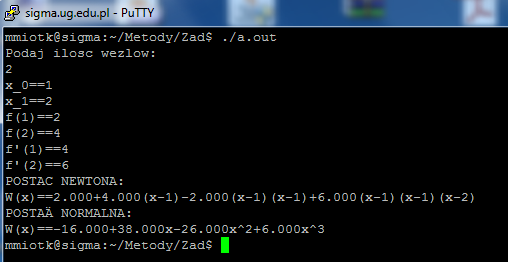
\includegraphics {obraz_nowy1.png}\\
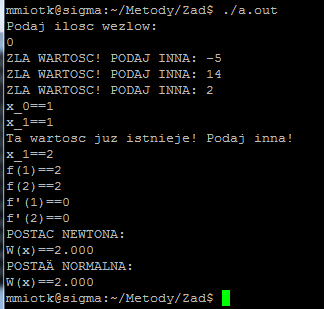
\includegraphics{obraz_nowy2.png}\\
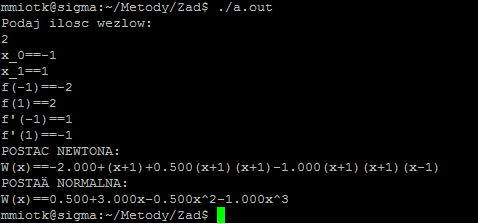
\includegraphics{obraz_nowy3.png}
\end{document}
